\section{Results}
\label{sec:results}

\subsection{Target-specific risks under known truth}
\label{sec:res-theory}

The known-truth simulation reproduced the qualitative separation implied by the model (Fig.~\ref{fig:concept}). With a fixed, correctly known reporting probability, error about the current reproduction number decreased with inverse case volume. Error about a fixed collection of realised reproduction numbers also decreased, because those realised fluctuations were part of the target rather than an error component. At a fixed number of sampled periods, error about the stationary process mean retained the variance of the realised mean. The simulation checks these formulas under their own assumptions; it is not evidence that an empirical admission-statistic intercept has the same origin.

When the estimate used the mean reporting probability while period-specific completeness fluctuated independently, current-value error approached the reporting term rather than zero. The finite-period mean inherited a reporting contribution divided by the number of independent periods. Thus the absence of an environmental floor for a realised target did not imply the absence of an observation-process floor. Simulation records include Monte Carlo standard errors for each comparison, so numerical differences are judged against simulation uncertainty rather than an arbitrary percentage agreement. The variance balance and budget examples in Appendix~\ref{app:extensions} refer to this specified model, not to operational thresholds inferred from admissions.

\begin{figure}[tbp]
\centering
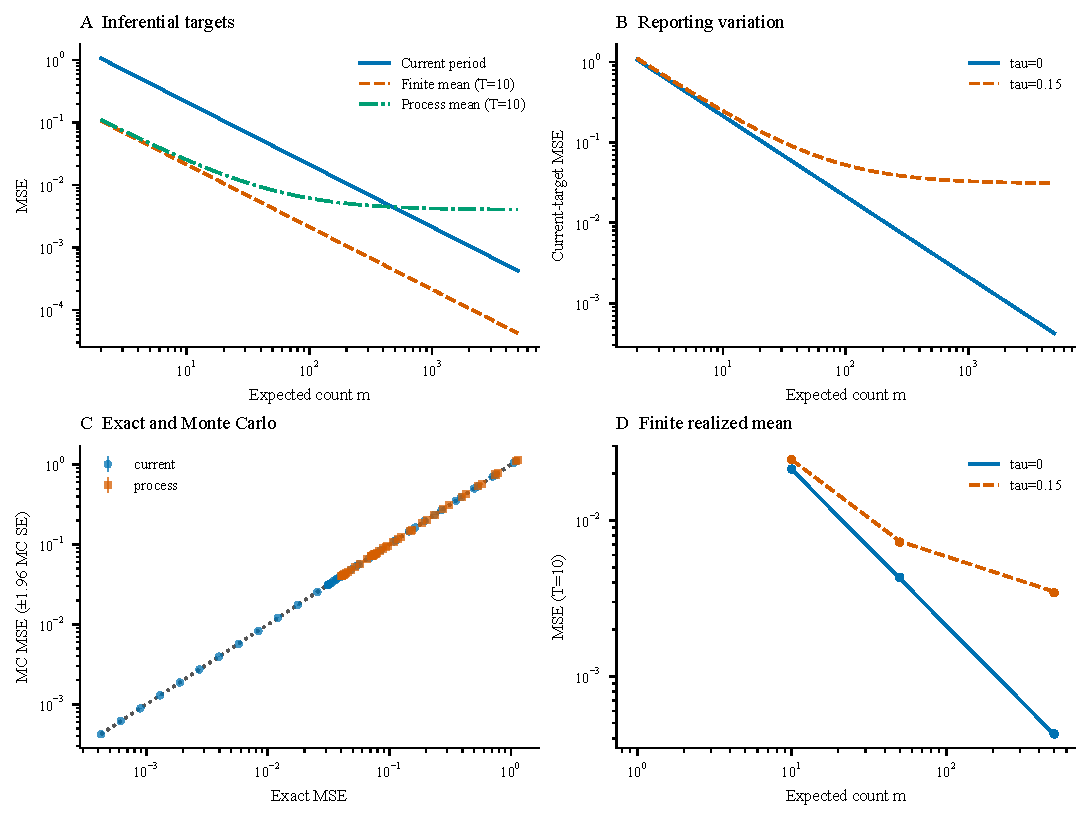
\includegraphics[width=\linewidth]{figures/fig_01_targets.pdf}
\caption{Inferential targets and reporting assumptions. Curves give the model risks and points, where shown, give known-truth Monte Carlo checks. Current-value and realised finite-period targets differ from the stationary process mean. Unobserved period-level reporting variation can leave a nonzero risk even for current values. Counts are generated under the stated fixed-exposure model; the figure does not identify a biological variance floor in the hospital data.}
\label{fig:concept}
\end{figure}

\subsection{Observed loss curves and held-out comparison}
\label{sec:res-empirical}

The rebuilt primary $R_A$ sample contained \Nra{} state-weeks. The affine working fit gave $a=\RAaPoint{}$ (95\% interval \RAaInterval{}), $b=\RAbPoint{}$ (\RAbInterval{}) and an apparent ratio $b/a=\RAratioPoint{}$ (\RAratioInterval{}). The corresponding ratio for $G$ was \GratioPoint{} (\GratioInterval{}; Table~\ref{tab:pooled}). These are estimates of the apparent statistics' relative dispersion under the specified affine form. A positive conditional intercept does not establish the form of the curve outside the observed count range.

The two fitted curves described similar broad changes over the observed support, but their held-out rankings were not uniform (Fig.~\ref{fig:model-comparison}; Table~\ref{tab:cv}). For $R_A$, the average power-law-minus-affine score was \RAstateCVPoint{} when leaving out states and \RAseasonCVPoint{} when leaving out seasons. The negative state score favoured the power law, while the positive season score favoured the affine model. For $G$, both summaries favoured the power law (\GstateCVPoint{} and \GseasonCVPoint{}). These comparisons now use training-fold centres throughout. Individual fold values are provided because a small aggregate difference conceals variation between held-out settings, and the four season folds supply little information about generalisation to new epidemic regimes.

Neither the fitted positive intercept nor this mixed predictive comparison provides independent evidence for an invariant transmission-variance floor. We therefore retain $b/a$ only as an affine descriptive ratio. The 3.2-day transform sensitivities in Table~\ref{tab:pooled} preserve the distinction between a changed apparent statistic and a change in the true interval assumed by a simulator. They do not identify which interval generated the observed admissions. The supplementary design experiment evaluates distinguishability under declared synthetic curves; its high power in some settings is not substituted for an empirical test, and its held-out null rejection rates are reported alongside power.

\begin{figure}[tbp]
\centering
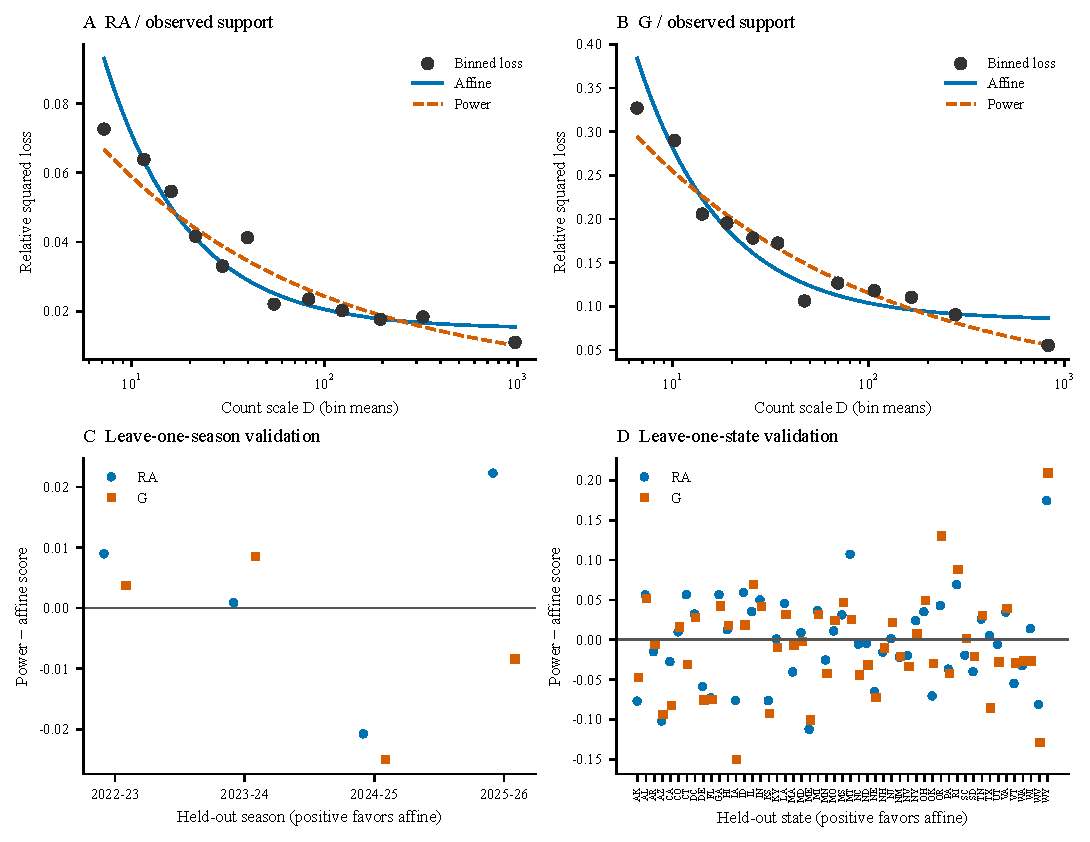
\includegraphics[width=\linewidth]{figures/fig_02_models.pdf}
\caption{Empirical support and held-out curve comparison. Binned means describe relative loss over observed case counts; they are not independent observations and are not used as an unclustered significance test. The affine and power-law curves are fitted working means. Held-out score differences use centres and model parameters estimated within training folds. Positive power-law-minus-affine differences favour the affine model; negative differences favour the power law. Fold scores do not constitute independent replications.}
\label{fig:model-comparison}
\end{figure}

\subsection{Response to controlled removal of cases}
\label{sec:res-thinning}

For the $R_A$ sample (n=\Nra{} state-weeks), across all retention levels the fitted thinning rate was \ThinAllPoint{} (95\% interval \ThinAllInterval{}), against the approximate elasticity reference \ThinBPPoint{}. Its paired ratio to that reference was \ThinRatioPoint{} (\ThinRatioInterval{}). Excluding the most extreme retention level gave \ThinNoqPoint{} (\ThinNoqInterval{}; Fig.~\ref{fig:thinning}, Table~\ref{tab:thinning}). The contrast between these summaries matters because the $q=0.1$ point supplies about 76\% of the through-origin predictor sum of squares. This leverage is a property of the chosen inverse-retention design, not by itself proof that the observation is biased.

The original-$C_t\ge50$ subset gave \ThinHighPoint{} (\ThinHighInterval{}), while requiring both current and next counts to be at least 50 gave \ThinBothPoint{} (\ThinBothInterval{}). The latter restriction addresses a limitation of the first: a large current count does not ensure a large numerator after thinning. All these subsets were defined from original counts, with no post-thinning reselection. Their different reference coefficients are recomputed rather than borrowing the full-sample reference.

Figure~\ref{fig:thinning} also shows changes in intercept and their joint uncertainty. These changes, including any departure at low retention, are part of the result. A confidence interval containing zero is not evidence of exact intercept invariance. The nonlinear transformation, continuity correction, recentering and refitting can modify the response even when the imposed count-removal mechanism is known. The known Poisson-count check in the supplementary output examines that complete pipeline, without claiming to represent every reporting mechanism in practice.

The calculation used \ThinBootstrap{} outer samples, \ThinPointReps{} point realisations and \ThinInnerReps{} inner realisations per bootstrap level. Numerical precision is documented in Table~\ref{tab:thinning}, including the predefined Monte Carlo check and fit failures. Because the point estimate averages more realisations than each bootstrap draw, the interval includes both sampling and finite-inner simulation variation; Table~
ef{tab:thinning} reports the two components separately. The experiment establishes how these recorded counts respond to additional random removal. It does not separate transmission, admission practice, delayed observation and reporting variation in the original intercept, nor does the difference between $b(1)$ and $c_{\rm thin}$ uniquely quantify offspring overdispersion.

\begin{figure}[tbp]
\centering
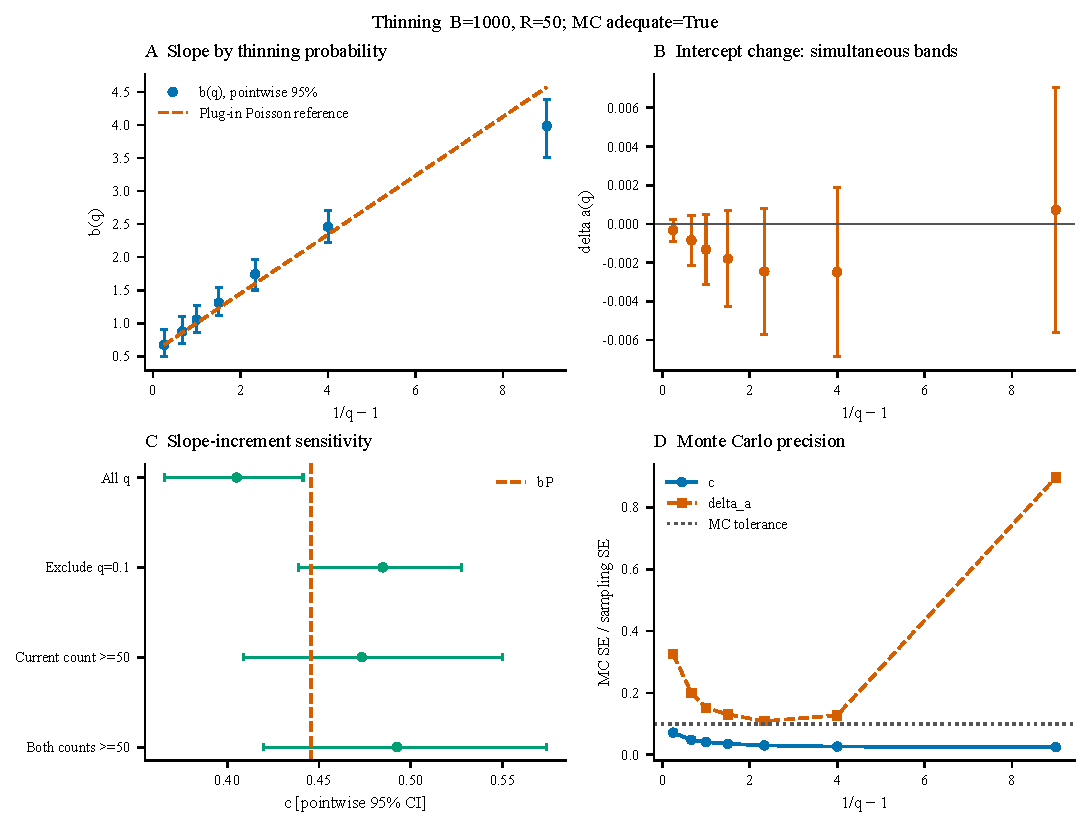
\includegraphics[width=\linewidth]{figures/fig_03_thinning.pdf}
\caption{Controlled thinning on the frozen sample. Coefficients are fitted on the original count scale after recomputing the statistic and its centre. Intercept-change bands account for their joint bootstrap variation across retention levels. Sensitivity summaries retain all levels, omit $q=0.1$, or restrict the original current and next counts. The Poisson elasticity coefficient is an approximate reference, not an exact prediction for every nonlinear fitted coefficient. Actual inner and outer repetition counts are reported in Table~\ref{tab:thinning}.}
\label{fig:thinning}
\end{figure}

\subsection{State heterogeneity and the choice of loss reference}
\label{sec:res-fe}

For the same $R_A$ sample, with state intercepts and a shared within-state slope, $b_{\rm w}=\FEbPoint{}$ (\FEbInterval{}) and the mean state intercept was \FEaPoint{} (\FEaInterval{}). The mean-based ratio was \FEratioPoint{} (\FEratioInterval{}), and replacing the scale by the actual weighted $D_t$ gave \FEDratioPoint{} (\FEDratioInterval{}; Fig.~\ref{fig:heterogeneity}, Table~\ref{tab:fe}). The latter is a distinct fit, not an alias of the single-week count analysis.

The pooled-to-within-state paired ratio was \FEpairedPoint{} (\FEpairedInterval{}) under independent resampling of calendar weeks. The two- and three-week block intervals were \FEpairedBlockTwoInterval{} and \FEpairedBlockThreeInterval{}, respectively. The ordinary interval excluded one narrowly, whereas the time-block intervals included it. Consequently, the apparent difference is sensitive to how temporal dependence is represented. It cannot be translated into a causal percentage attributable to spatial averaging. The primary state model supplied \FEvalid{} valid fits among \FEBootstrap{} bootstrap samples; the conditional nature of finite-fit intervals and the diagnostic failures are explicit. The state-plus-week point diagnostic did not meet the numerical convergence criterion and is not assigned a slope or confidence interval.

Changing the reference of the loss also changed the intercept (Table~\ref{tab:centering}). With the common global denominator retained, replacing the pooled centre by the national-week centre reduced the $R_A$ intercept by \RAweekReductionPoint{}\% (\RAweekReductionInterval{}\%) and the $G$ intercept by \GweekReductionPoint{}\% (\GweekReductionInterval{}\%). The reduction is specific to holding the denominator fixed; changing the normalisation as well would define a different, non-comparable quantity. Season centring and common linear detrending did not reproduce that same change. This is expected: different references remove different components of the observed trajectory, including genuine common signal. The leave-own-state-out variant documents the influence of using an observation in its own weekly reference. These comparisons describe specification sensitivity, not an identified decomposition into independent transmission and reporting variances.

\begin{figure}[tbp]
\centering
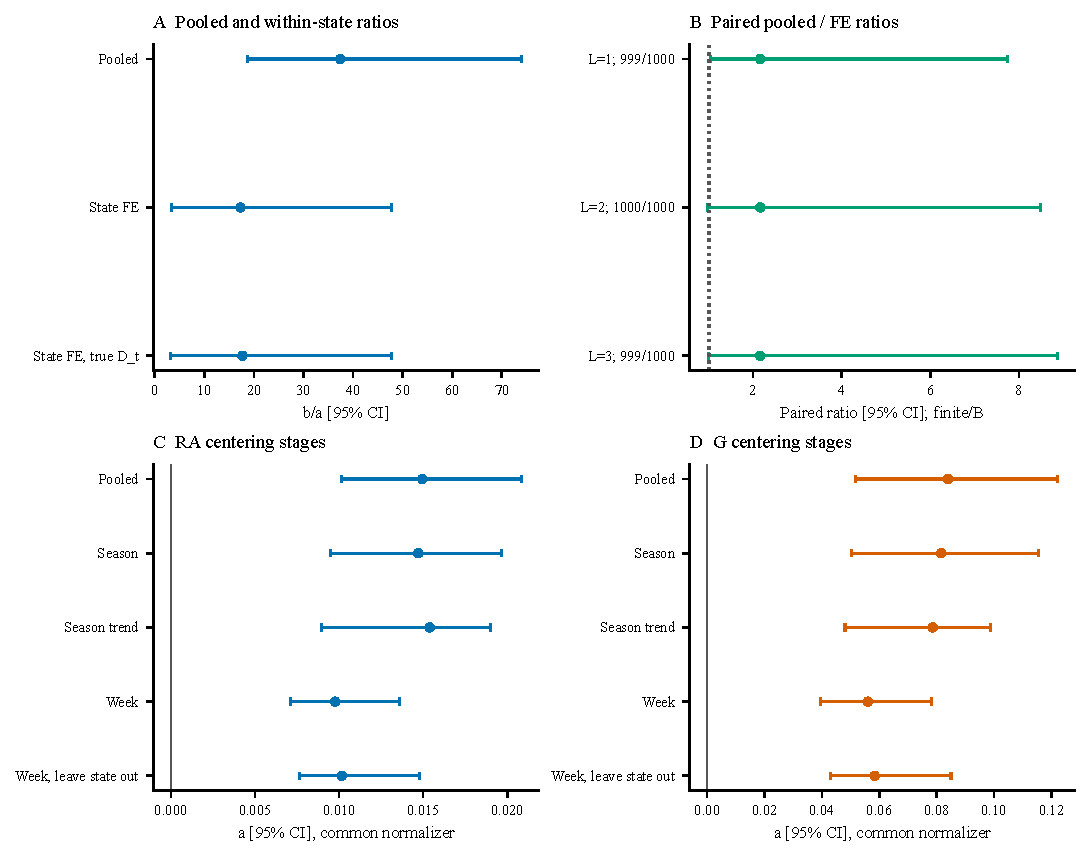
\includegraphics[width=\linewidth]{figures/fig_04_heterogeneity.pdf}
\caption{Spatial specification and reference sensitivity. Pooled and state-intercept estimates use the same underlying global-loss definition; the $D_t$ sensitivity uses the weighted lagged count. Reference adjustments hold the global normalisation fixed and change the centre or common trend. Time-block paired intervals show sensitivity to the treatment of temporal dependence. Undefined or unconverged quantities are not drawn as successful estimates. Different references define different empirical targets.}
\label{fig:heterogeneity}
\end{figure}

\subsection{Limits of the conditional calibration}
\label{sec:res-sim}

The supplementary calibration applies the corrected observation mechanism to both apparent statistics and reports all declared scenarios (Table~\ref{tab:calibration}). It distinguishes the source-matched 3.2-day, SD 2.1-day interval from a fixed-coefficient-of-variation sensitivity and the historical 3.6-day proxy. Conditional intervals combine paired empirical and simulator uncertainty; they do not average over an invented distribution of interval assumptions.

A simulator can reproduce an intercept while failing to reproduce the slope or retained sample size. Those discrepancies are therefore retained in the response checks rather than eliminated by adjusting initial zero counts or selecting a preferred scenario. The initial-condition and no-importation assumptions can leave initially zero states without subsequent infections, which differs from surveillance settings with continuing introductions. National and state persistence, count overdispersion and reporting volatility are likewise separate mechanisms in the checked simulator. Multiple compatible summaries would not identify one of them uniquely. No calibrated value is used here to claim that a fixed proportion of real state-weeks exceeds a biological or economic threshold.
